\documentclass[10pt,a4paper]{article}
\usepackage[utf8]{inputenc}
\usepackage{amsmath}
\usepackage{amsfonts}
\usepackage{amssymb}
\usepackage{graphicx}
\usepackage{tabularx}

\begin{document}
\newcolumntype{R}{>{\raggedright\arraybackslash}X}
\section{Johdanto}
\subsection{Ohjelman kuvaus}
Tarkoitus on toteuttaa web-sovellus, joka mahdollistaa tiedostojen lataamisen palvelimelle ja palvelimelta. Palvelimella olevia tiedostoja voi kommentoida. Tiedostoihin liittyy myös teemasanoja, joiden perusteella tiedostoja voi hakea. Käyttäjät voivat rekisteröityä palveluun, mutta se ei ole pakollista. Kaikki käyttäjät voivat lisätä tiedostoja ja viestejä. Rekisteröityneet käyttäjät voivat lisäksi muokata tai poistaa lisäämiään tiedostoja tai viestejä.

\subsection{Toteutus- ja toimintaympäristö}
Sovellus toteutetaan PHP:llä ja se toimii Helsingin yliopiston users-palvelimella. Sovellus käyttää PostgreSQL-tietokantaa.

\section{Käyttötapaukset}
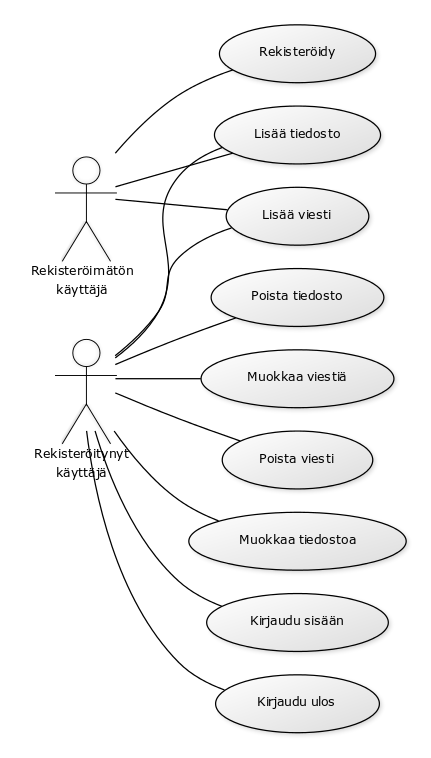
\includegraphics[scale=0.7]{kaaviot/kayttotapauskaavio.png}
\subsection{Käyttäjäryhmät}
\paragraph{Rekisteröimätön käyttäjä}
Kuka tahansa web-käyttäjä. Tunnistautumaton käyttäjä.

\paragraph{Rekisteröitynyt käyttäjä}
Käyttäjä, joka on luonut tunnukset sivulle. Tunnistautunut käyttäjä.

\subsection{Käyttötapaukset käyttäjäryhmittäin}
\subsubsection{Rekisteröimätön käyttäjä}
\paragraph{Lisää tiedosto}
Käyttäjä lisää tiedoston palvelimelle.
\paragraph{Lisää viesti}
Käyttäjä lisää viestin johonkin tiedostoon liittyen.

\paragraph{Rekisteröidy}
Luodaan käyttäjälle käyttäjätunnus. Tämän jälkeen käyttäjä voi kirjautua järjestelmään.
\paragraph{Kirjaudu sisään}
Käyttäjä tunnistautuu järjestelmään.


\subsubsection{Rekisteröitynyt käyttäjä}
\paragraph{Lisää tiedosto}
Käyttäjä lisää tiedoston palvelimelle.
\paragraph{Muokkaa tiedostoa}
Tiedostoon liittyvää metatietoa, kuten nimeä tai kuvausta, voi muokata. Tiedoston sisältöä ei voi muokata.
\paragraph{Poista tiedosto}
Käyttäjän valitsema ja omistama tiedosto poistetaan. Tiedostoon liittyvät viestit ja metatiedot poistetaan myös.

\paragraph{Lisää viesti}
Käyttäjä lisää viestin johonkin tiedostoon liittyen.
\paragraph{Muokkaa viestiä}
Rekisteröitynyt käyttäjä voi muokata minkä tahansa lähettämänsä viestin sisältöä, aihetta tai muita tietoja.
\paragraph{Poista viesti}
Käyttäjän valitsema ja omistama viesti poistetaan.

\paragraph{Kirjaudu ulos}
Käyttäjä kirjataan ulos.

\section{Järjestelmän tietosisältö}
\subsection{Käsitekaavio}
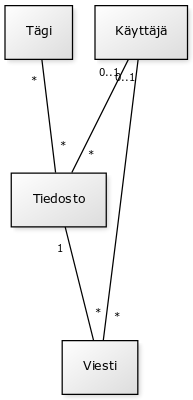
\includegraphics[scale=0.7]{kaaviot/kasitekaavio.png}
\subsection{Käsitteiden attribuutit}
\subsubsection{Käyttäjä}
\begin{tabularx}{\textwidth}{|R|R|R|} \hline
\textbf{Attribuutti} & \textbf{Arvojoukko} & \textbf{Kuvailu}\\ \hline
Käyttäjänimi & Merkkijono max. 50 merkkiä & Käyttäjän rekisteröitymisen yhteydessä valitsema käyttäjänimi\\ \hline
Salasanatiiviste & Merkkijono & Käyttäjän salasanasta tehty tiiviste\\ \hline
\end{tabularx}

\subsubsection{Tiedosto}
\begin{tabularx}{\textwidth}{|R|R|R|} \hline
\textbf{Attribuutti} & \textbf{Arvojoukko} & \textbf{Kuvailu}\\ \hline
Tiedoston lisääjä & Käyttäjä & Käyttäjä, joka latasi tiedoston palvelimelle\\ \hline
Tiedostonimi & Merkkijono & Tiedoston nimi\\ \hline
Tiedoston kuvaus & Merkkijono & Kuvaus tiedoston sisällöstä, konteksti tiedostolle\\ \hline
Aikaleima & Aikaleima ja aikavyöhyke & Aika, jolloin tiedosto ladattiin palvelimelle\\ \hline
Tiedostopolku & Merkkijono & Polku tiedostoon tiedostojärjestelmässä\\ \hline
Tiedoston koko & Kokonaisluku & Tiedoston koko tavuina\\ \hline
Tiedostotyyppi & Merkkijono & Tiedoston MIME-tyyppi esim. text/plain\\ \hline
\end{tabularx}

\subsubsection{Tägi}
\begin{tabularx}{\textwidth}{|R|R|R|} \hline
\textbf{Attribuutti} & \textbf{Arvojoukko} & \textbf{Kuvailu}\\ \hline
Tägin nimi & Merkkijono & Nimi joka näytetään tiedoston yhteydessä ja jolla tiedostoja haetaan\\ \hline
Tägin kuvaus & Merkkijono & Taustatietoa tagista, konteksti, milloin käytetään jne.\\ \hline
\end{tabularx}

\subsubsection{Viesti}
\begin{tabularx}{\textwidth}{|R|R|R|} \hline
\textbf{Attribuutti} & \textbf{Arvojoukko} & \textbf{Kuvailu}\\ \hline
Viestin lisääjä & Käyttäjä & Käyttäjä, joka kirjoitti viestin\\ \hline
Tiedosto & Tiedosto & Tiedosto, johon viesti liittyy\\ \hline
Aihe & Merkkijono & Viestin aihe, otsikko\\ \hline
Leipäteksti & Merkkijono & Viestin varsinainen sisältö\\ \hline
Aikaleima & Aikaleima ja aikavyöhyke & Aika, jolloin viesti saapui palvelimelle\\ \hline
\end{tabularx}

\section{Relaatiotietokantakaavio}
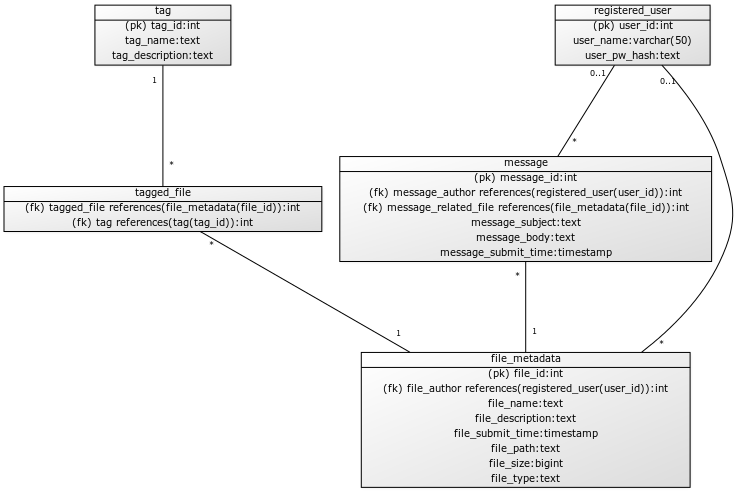
\includegraphics[scale=0.5]{kaaviot/tietokantakaavio.png}
\end{document}
